\documentclass[notheorems, handout]{beamer}

\usetheme{Warsaw}
\setbeamertemplate{page number in head/foot}[totalframenumber]
\setbeamertemplate{headline}{}
\setbeamertemplate{navigation symbols}{}
\usefonttheme[onlymath]{serif}

\usepackage[utf8]{inputenc}
\usepackage[T2A]{fontenc}
\usepackage[russian]{babel}

\usepackage{graphicx,subcaption,ragged2e}
\usepackage{tikz}
\usepackage{bm}
\usepackage{amsfonts}

\newtheorem{theorem}{Теорема}
\newtheorem{definition}{Определение}
\newtheorem{remark}{Замечание}

\title[Статистическое и машинное обучение]{Решающие деревья. Random
Forest. Бустинг.}

\institute[Санкт-Петербургский Государственный Университет]{%
  \small
  Санкт-Петербургский государственный университет\\
  Кафедра статистического моделирования
}

\date[Сентябрь 2025]{Санкт-Петербург, 2025}

\begin{document}

\begin{frame}
  \titlepage
\end{frame}

\begin{frame}{Решающие деревья}
  \textbf{Решающее дерево}~--- это бинарное дерево, где
  \begin{itemize}
    \item во всех внутренних вершинах $v$ задан некоторый предикат
      $\beta_{v}: \mathbf{X} \to {0{,} 1}$,
    \item в каждой листовой вершине $v$ задан прогноз $c_{v} \in
      \mathbf{Y}$ (для классификации возможно: $c_{v} \in
        \mathbb{R_{+}^{K}}$, \; $\displaystyle\sum_{k = 1}^{K}
      c_{v_{k}} = 1$~--- вектор вероятностей принадлежности к классу).
  \end{itemize}
  \par\smallskip
  \begin{figure}[h!]
    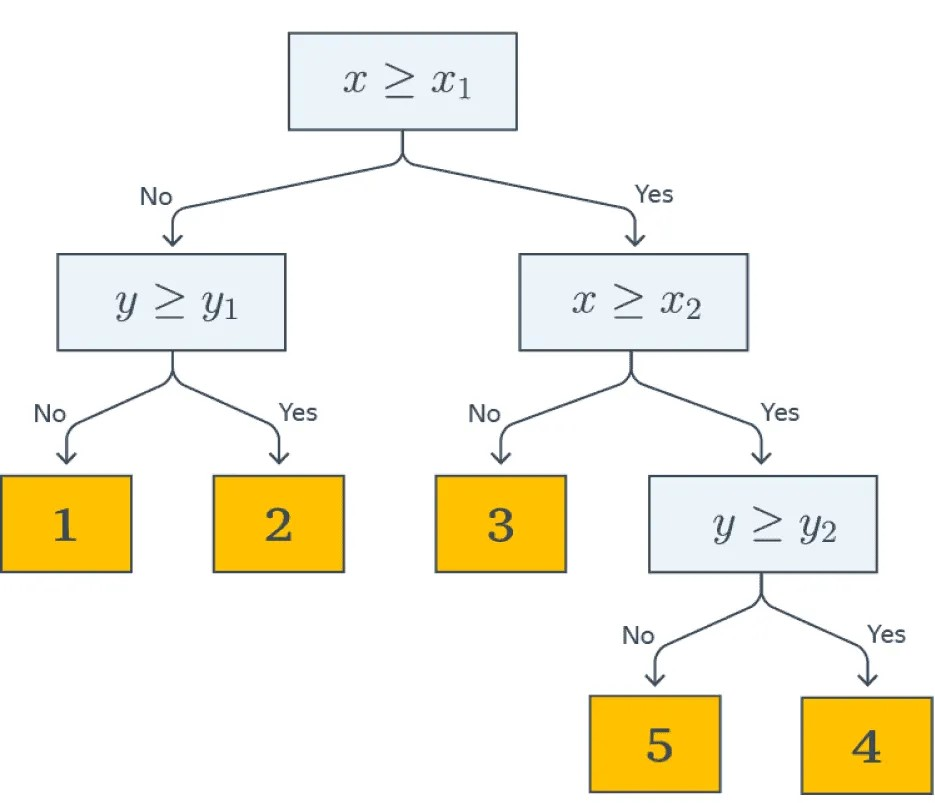
\includegraphics[width=0.4 \textwidth]{img/detree}
    \caption{Решающее бинарное дерево}
  \end{figure}
\end{frame}

\begin{frame}{Постановка задачи}
  Решающие деревья можно применять как для задач регрессии,
  так и для задач классификации.
  \par\smallskip
  Пусть $\mathbf{X}$~--- множество объектов, $\mathbf{Y}$~---
  множество ответов, $y: \mathbf{X} \to \mathbf{Y}$~--- некоторая зависимость.
  \par\smallskip
  Есть обучающая выборка $\mathbf{D} = \{(x_{i}{,} \; y_{i})\}_{i =
  1}^{n}$, где $x_{i}$~--- входные данные, $y_{i}$~--- известные ответы.
  \par\smallskip
  \begin{itemize}
    \item $y_{i} \in \{1{,}\dots{,}\;K\} \Rightarrow$ задача классификации.
    \item $y_{i} \in \mathbb{R} \Rightarrow$ задача регрессии.
  \end{itemize}
\end{frame}

\begin{frame}{Решающие деревья в задаче регрессии}
  Пусть $\mathbf{X} \in \mathbb{R}^{n \times p}$~--- матрица данных
  (где $p$~--- признаки, $n$~--- наблюдения), $\mathbf{Y} \in
  \mathbb{R}^{n}$~--- отклик.
  \par\smallskip
  \textbf{Идея}: разбиение совокупности всех возможных значений
  $\mathbf{X}_{1}, \dots{,}\; \mathbf{X}_{p}$ на $J$ непересекающихся
  областей $R_{1}, \dots{,}\; R_{J}$.
  \par\smallskip
  Предсказание для объекта $x$:
  \begin{flalign*}
    f(x) = \displaystyle\sum_{j = 1}^{J} c_{j} \mathbf {1}(x \in R_{j}).
  \end{flalign*}
  Многомерные прямоугольники $R_{1}, \dots{,}\; R_{J}$ выбираем так,
  чтобы минимизировать сумму квадратов остатков:
  \begin{flalign*}
    RSS = \displaystyle\sum_{j = 1}^{J}\displaystyle\sum_{i \in
    \mathbf{R}_{j}}{(y_{i} - f(x_{i}))}^{2} \rightarrow \min_{R_{1},
    \dots{,}\; R_{J}}.
  \end{flalign*}
  Тогда
  \begin{flalign*}
    \hat{c}_{j} = \frac{1}{|R_{j}|} \displaystyle\sum_{x_{i} \in R_{j}} y_{i}.
  \end{flalign*}
\end{frame}

\begin{frame}{Решающие деревья в задаче регрессии}
  \begin{figure}[h!]
    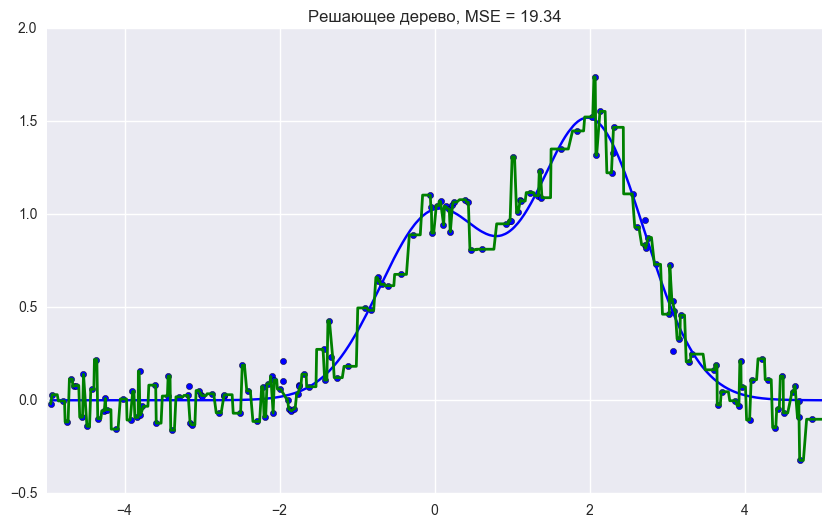
\includegraphics[width=1 \textwidth]{img/retree}
    \caption{Плохо обобщает закономерность и более склонна к переобучению}
  \end{figure}
\end{frame}

\begin{frame}{Решающие деревья в задаче классификации}
  В задаче классификации $R_{1}, \dots{,}\; R_{J}$ минимизируется
  число ошибок классификации
  \begin{flalign*}
    M(j) = 1 - \max_{k}(\hat{p}_{jk}),
  \end{flalign*}
  где $\hat{p}_{jk}$~--- доля объектов обучающей выборки класса $k$
  попавших в $R_{j}$.
  \par\smallskip
  На практике чаще используют две других метрики:
  \begin{itemize}
    \item $G(j) = \displaystyle\sum_{k = 1}^{K} \hat{p}_{jk} (1 -
      \hat{p}_{jk})$~--- индекс Джини,
    \item $CI(j) = -\displaystyle\sum_{k = 1}^{K} \hat{p}_{jk}
      \log{\hat{p}_{jk}}$~--- коэффициент перекрестной энтропии.
  \end{itemize}
  Предсказание для объекта x:
  \begin{flalign*}
    f(x) = \underset{k \in \mathbf{Y}}{\operatorname{argmax}}\; \hat{p}_{jk}.
  \end{flalign*}
\end{frame}

\begin{frame}{Решающие деревья в задаче классификации}
  \begin{figure}[h!]
    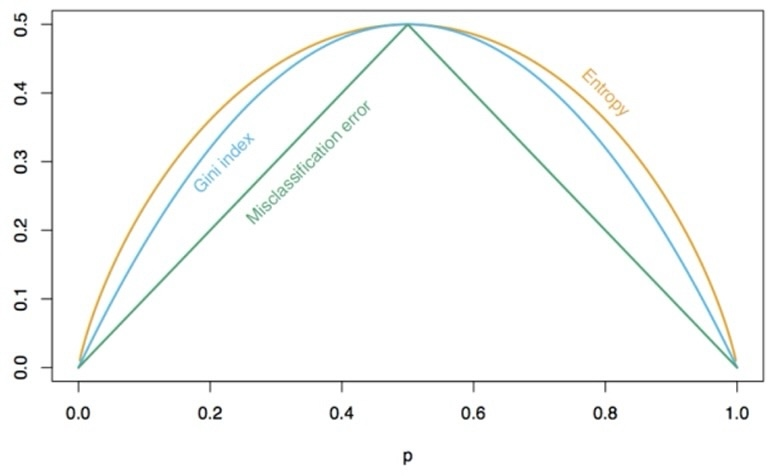
\includegraphics[width=1 \textwidth]{img/cltree1}
    \caption{Информационные индексы M, G, CI в случае двух классов}
  \end{figure}
\end{frame}

\begin{frame}{Решающие деревья в задаче классификации}
  \begin{figure}[h!]
    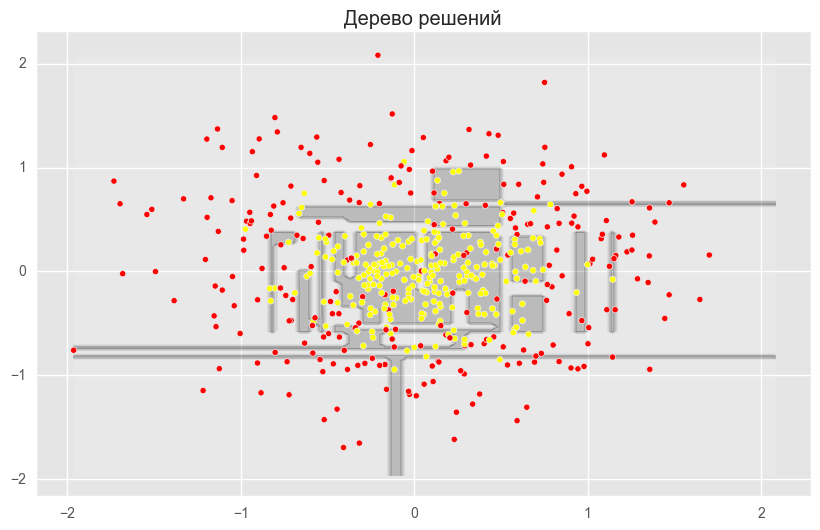
\includegraphics[width=0.9 \textwidth]{img/cltree2}
    \caption{Разделяющая граница дерева решений очень рваная и на ней
      много острых углов, что говорит о переобучении и слабой
    обобщающей способности}
  \end{figure}
\end{frame}

\begin{frame}{Жадный алгоритм построения решающего дерева}
  Нахождение оптимального дерева~--- это NP-полная задача.

  Пусть $X$~--- исходное множество обучающей выборки, а $X _m$ —
  множество объектов, попавших в текущий лист (в самом начале $X _m =
  X$). Тогда жадный алгоритм можно верхнеуровнево описать следующим образом:

  \begin{enumerate}
    \item Создаём вершину $v$;
    \item Если выполнен критерий остановки $\mathrm{Stop}(X _m)$, то
      останавливаемся, объявляем эту вершину листом и ставим ей в
      соответствие ответ $\mathrm{Ans}(X _m)$, после чего возвращаем её;
    \item Иначе: находим предикат $B _{j, t}$ (сплит), который
      определит наилучшее разбиение текущего множества объектов $X
      _m$ на две подвыборки $X _l$ и $X _r$, максимизируя критерий
      ветвления $\mathrm{Branch}(X _m, j, t)$;
    \item Для $X _l$ и $X _r$ рекурсивно повторим процедуру.
  \end{enumerate}

  На выходе получаем дерево, в каждом из листов которого содержится
  по крайней мере один объект исходной выборки.
\end{frame}

\begin{frame}{Значение листа}
  $\mathrm{Ans}(X _m)$ вычисляет ответ для листа по попавшим в него
  объектам из обучающей выборки. Может быть:\medskip

  \begin{enumerate}
    \item в случае задачи классификации — меткой самого частого
      класса или оценкой дискретного распределения вероятностей
      классов для объектов, попавших в этот лист;\medskip
    \item в случае задачи регрессии — средним, медианой или другой
      статистикой;\medskip
    \item простой моделью. К примеру, листы в дереве, задающем
      регрессию, могут быть линейными функциями или синусоидами,
      обученными на данных, попавших в лист.
  \end{enumerate}
\end{frame}

\begin{frame}{Критерии остановки}
  Критерий остановки $\mathrm{Stop}(X _m)$~--- функция, которая
  решает, нужно ли продолжать ветвление или пора остановиться.

  \begin{itemize}
    \item Ограничение максимальной глубины дерева.
    \item Ограничение минимального числа объектов в листе.
    \item Ограничение максимального количества листьев в дереве.
    \item Остановка в случае, если все объекты в листе относятся к
      одному классу.
    \item Остановка в случае, если изменение метрики меньше порога.
  \end{itemize}
  \begin{remark}
    Для очень глубоких деревьев имеем переобучение.
  \end{remark}
\end{frame}

\begin{frame}{Критерий ветвления}
  $\mathrm{Branch} (X _m, \text{feature}, \text{value})$~--- функция,
  измеряющая, насколько улучшится финальная метрика дерева при
  предлагаемом сплите.

  Пусть $L (y _i, c)$~--- функция потерь, $c$~--- константное
  предсказание. Информативность узла (хотим минимизировать):
  \[
    H (X _m) = \frac 1 {|X _m|} \sum _{(x _i, y _i) \in X _m} L (y _i, c).
  \]
  Если разделить на два узла:
  \[
    \begin{aligned}
      &\frac 1 {|X _m|} \left(\sum _{(x _i, y _i) \in X _l} L (y _i,
      c _l) + \sum _{(x _i, y _i) \in X _r} L (y _i, c)\right) =\\
      &= \frac {|X _l|} {|X _m|} H (X _l) + \frac {|X _r|} {|X _m|} H (X _r).
    \end{aligned}
  \]
\end{frame}

\begin{frame}{Критерий ветвления}
  Тогда критерий ветвления:
  \[
    \mathrm{Branch} (X _m, j, t) = |X _m| \cdot H(X _m) - |X _l|
    \cdot H(X _l) - |X _r| \cdot H(X _r).
  \]
  Чем больше изменение метрики, тем лучше.

  \begin{itemize}
    \item MSE: $L (y _i, c) = (y _i - c) ^2$, $H (X _m) = \sum
      \limits _{(x _i, y _i) \in X _m} \frac {(y _i - \overline{y})
      ^2} {|X _m|}$;
    \item MAE: $L (y _i, c) = |y _i - c|$, $H (X _m) = \sum \limits
      _{(x _i, y _i) \in X _m} \frac {|y _i - \mathrm{MEDIAN}(Y _m)|} {|X _m|}$;
    \item Для классификации можно рассматривать: misclassification
      error ($H (X _m) = 1 - \max p _i$, $p _i$~--- доля класса $i$),
      энтропию ($H (X _m) = - \sum ^K _{k = 1} p _k \log p_k$) или
      критерий Джини ($H (X _m) = \sum ^K _{k = 1} p _k (1 - p_k)$).
  \end{itemize}
\end{frame}

\begin{frame}{Стрижка деревьев(pruning tree)}
  \begin{itemize}
    \item \textbf{Проблема}: переобучение~--- небольшое смещение, но
      большая дисперсия.\medskip
    \item \textbf{Решение}: объединяя некоторые $R_{j}$ можем
      уменьшить дисперсию за счет небольшого увеличения смещения.\medskip
    \item Выращиваем дерево только до тех пор, пока уменьшение
      функции потерь из-за разбиения превышает некоторый (высокий)
      порог.\medskip
    \item Однако можно пропустить хорошее разбиение, остановившись
      слишком рано. Поэтому можно выращивать большие деревья $T_{0}$,
      а затем обрезать его для получения поддерева.\medskip
  \end{itemize}
\end{frame}

\begin{frame}{Cost-complexity pruning}
  \begin{itemize}
    \item Получим большое дерево $T_{0}$ и обрежем его в узле $t$,
      получив поддерево $T^{t} \subset T_{0}$.\medskip
    \item Рассмотрим последовательность деревьев проиндексированных
      положительным параметром $\alpha$. Каждому $\alpha$
      соответствует поддерево $T \subset T_{0}$, минимизирующее критерий
      \begin{flalign*}
        Q_{\alpha}(T) = Q(T) + \alpha |l(T)|,
      \end{flalign*}
      где $Q(T)$~--- разница между прогнозируемым и фактическим
      выходом модели на этапе её обучения, $\alpha \geq 0$,
      $|l(T)|$~--- число листьев в поддереве $T$.\medskip
    \item Выберем $\alpha$ с помощью кросс-валидации и возьмем
      соответствующее поддерево.
  \end{itemize}
\end{frame}

\begin{frame}{Преимущества и недостатки решающих деревьев}
  \textbf{Преимущества}:
  \begin{itemize}
    \item Простота интерпретации.
    \item Простота визуализации.
    \item Пригодность и для задач регрессии, и для задач классификации.
    \item Возможность работы с пропусками в данных.
    \item Возможность работы с категориальными значениями.
  \end{itemize}
  \par\smallskip
  \textbf{Недостатки}:
  \begin{itemize}
    \item Метод явялется неустойчивым и склонным к переобучению.
  \end{itemize}
  \par\smallskip
  \begin{remark}
    Агрегирования множества деревьев решений такими способами, как
    bagging, random forest и boosting, позволяет значительно улучшить
    качество предсказания.
  \end{remark}
\end{frame}

\begin{frame}{Bootstrap}
  Метод бутстрэпа заключается в следующем:
  \begin{itemize}
    \item Дана выборка $\mathbf{X}$ размера $M$.
    \item Равномерно возьмем из выборки $M$ объектов с возвращением
      (из-за возвращения среди них окажутся повторы), обозначим новую
      выборку через $\mathbf{X}_{1}$.
    \item Повторив $N$ раз, сгенерируем N подвыборок
      $\mathbf{X}_{1}{,} \dots{,}\; \mathbf{X}_{N}$.
  \end{itemize}
  \par\smallskip
  \begin{figure}[h!]
    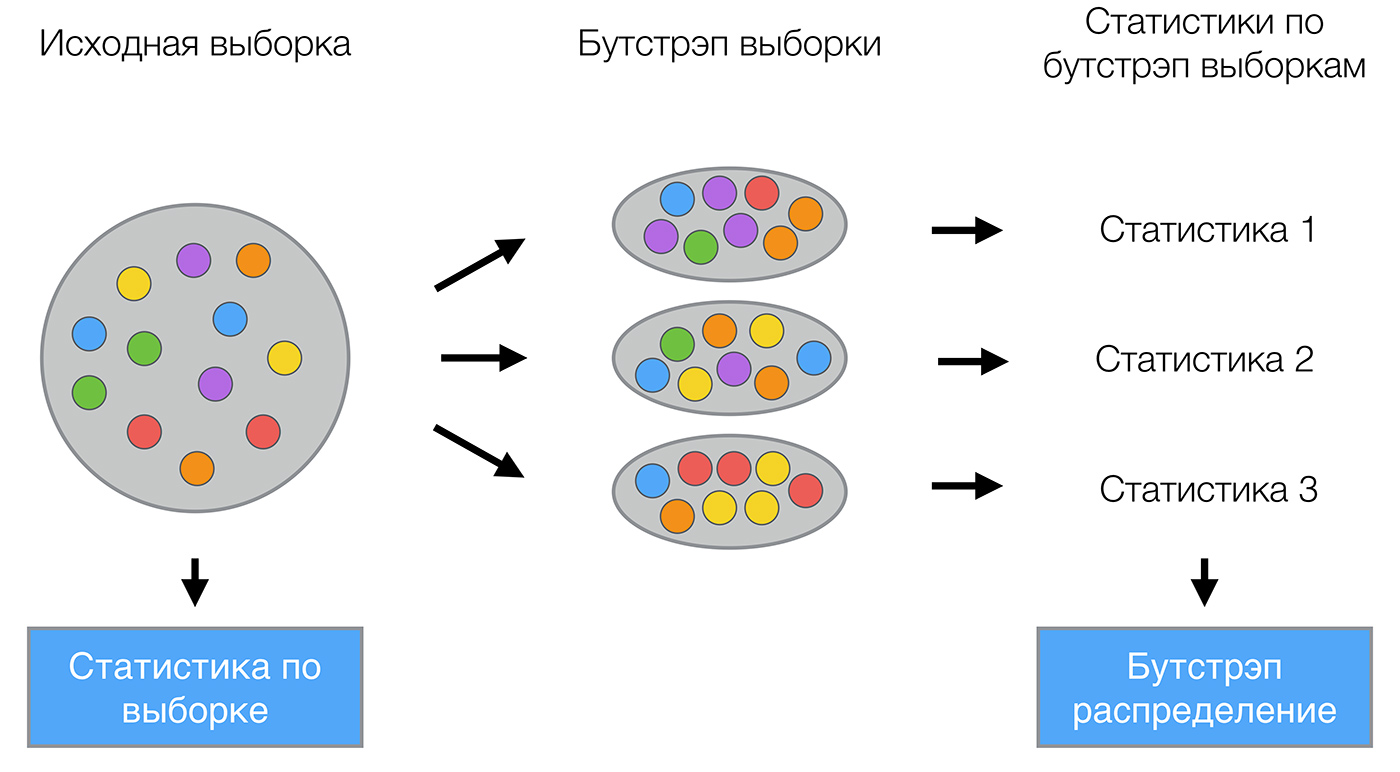
\includegraphics[width=0.7 \textwidth]{img/bootstrap}
  \end{figure}
\end{frame}

\begin{frame}{Пример построения композиции алгоритмов.}
  \begin{itemize}
    \item Дана конечная выборка $\mathbf{X} = (x_{i}{,}\;y_{i})$ с
      вещественными ответами.
    \item Равномерно возьмем из выборки $l$ объектов с возвращением
      (из-за возвращения среди них окажутся повторы), обозначим новую
      выборку через $\mathbf{X}_{1}$.
    \item Повторив $N$ раз, сгенерируем N подвыборок
      $\mathbf{X}_{1}{,} \dots{,}\; \mathbf{X}_{N}$.
    \item Обучим по каждой из  них линейную модель регрессии, получив
      базовые алгоритмы $b_{1}(x), \dots,\; b_{N}(x)$.
    \item Пусть $\exists$ модель $y(x) = \displaystyle\sum
      \beta_{i}x_{i} + \varepsilon_{i}$ и $p(x)$~--- распределение $\mathbf{X}$.
    \item \textbf{Ошибка каждой функции регрессии}:
      $\varepsilon_{j}(x) = b_{j}(x) - y(x)$, $\;j = 1, \dots,\;N$.
    \item \textbf{Матожидание среднеквадратичной ошибки}:
      $\mathbf{E}_{x}{(b_{j}(x) - y(x))}^{2} =
      \mathbf{E}_{x}\varepsilon_{j}^{2}(x)$.
  \end{itemize}
\end{frame}

\begin{frame}{Среднеквадратичная ошибка}
  Средняя ошибка построенных функций регрессии:
  \begin{flalign*}
    \mathbf{E}_{1} = \frac{1}{N} \displaystyle\sum_{j =
    1}^{N}\mathbf{E}_{x}\varepsilon_{j}^{2}(x).
  \end{flalign*}
  \par\smallskip
  Пусть ошибки несмещены и некоррелированы:
  \begin{flalign*}
    \mathbf{E}_{x}\varepsilon_{j}(x) = 0, \;\;\;
    \mathbf{E}_{x}\varepsilon_{j}(x)\varepsilon_{j}(x) = 0, \;\;\; i \neq j.
  \end{flalign*}
  \par\smallskip
  Построим теперь новую функцию регрессии, которая будет усреднять
  ответы построенных нами функций:
  \begin{flalign*}
    \alpha(x) = \frac{1}{N}\displaystyle\sum_{j = 1}^{N}b_{j}(x).
  \end{flalign*}
  \par\smallskip
  Тогда
  \begin{flalign*}
    E_{N} = \mathbf{E}_{x}{\left(\frac{1}{N} \displaystyle\sum_{j =
    1}^{N}b_{j}(x) - y(x)\right)}^{2} =
    \mathbf{E}_{x}{\left(\frac{1}{N} \displaystyle\sum_{j =
    1}^{N}\varepsilon_{j}(x)\right)}^{2} =
  \end{flalign*}
\end{frame}

\begin{frame}{Среднеквадратичная ошибка}
  \begin{flalign*}
    = \frac{1}{N^{2}}\mathbf{E}_{x}\left(\displaystyle\sum_{j =
      1}^{N}\varepsilon_{j}^{2}(x) + \displaystyle\sum_{i \neq
    j}\varepsilon_{i}(x)\varepsilon_{j}(x)\right) = \frac{1}{N}E_{1}.
  \end{flalign*}
  \par\smallskip
  Таким образом, усреднение ответов позволило уменьшить средний
  квадрат ошибки в $N$ раз (при этом смещение остаётся тем же).
  \par\smallskip
  \begin{remark}
    Рассмотренный пример не очень применим на практике, так как мы
    предположили, что ошибки некоррелированы, это редко выполняется.
    Если это предположение неверно, то уменьшение ошибки оказывается
    не таким значительным.
  \end{remark}
\end{frame}

\begin{frame}{Bagging}
  \textbf{Bagging}~--- метод, который позволяет уменьшить разброс
  модели. Этот метод обучает некоторое число алгоритмов так, что
  каждый алгоритм обучается на отдельных выборках, которые получены
  из исходной с помощью bootstrap.
  \begin{figure}[h!]
    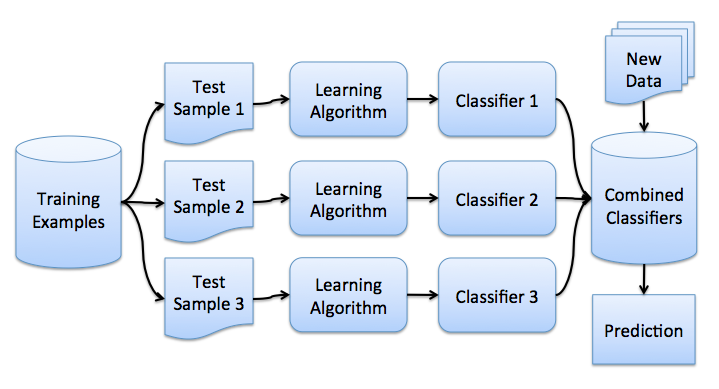
\includegraphics[width=0.9 \textwidth]{img/bagging}
    \caption{Схема реализации bagging}
  \end{figure}

\end{frame}

\begin{frame}{Реализация bagging}
  Пусть имеется обучающая выборка $\mathbf{X}$.
  \begin{enumerate}
    \item С помощью bootstrap сгенерируем из $\mathbf{X}$ выборки
      $\mathbf{X}_{1}, \dots,\; \mathbf{X}_{N}$.
    \item На каждой выборке строим решающее дерево $b_{n}(x)$:
      \begin{itemize}
        \item дерево строится, пока в каждом листе не окажется не
          более $n_{\min}$ объектов.
        \item при каждом разбиении сначала выбирается $m$ случайных
          признаков из $p$, оптимальное разделение ищется только среди них.
      \end{itemize}
    \item находим оценку:
      \begin{itemize}
        \item для задачи регрессии: $\alpha(x) =
          \frac{1}{N}\displaystyle\sum_{n = 1}^{N} b_{n}(x)$.
        \item для задачи классификации с $K$ классами: записываем
          класс предсказанный каждым деревом, итоговое предсказание
          часто встречающийся класс среди предсказаний.
      \end{itemize}
  \end{enumerate}
\end{frame}

\begin{frame}{Bagging в задаче регрессии}
  \begin{figure}[h!]
    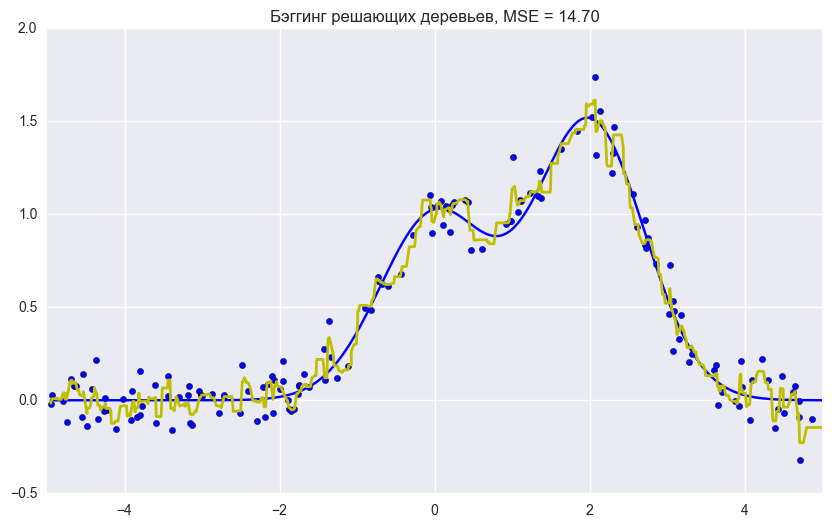
\includegraphics[width=1 \textwidth]{img/bagging_re}
    \caption{Лучше обобщает закономерность и менее склонна к
    переобучению, чем любое отдельное дерево}
  \end{figure}
\end{frame}

\begin{frame}{Bagging в задаче классификации}
  \begin{figure}[h!]
    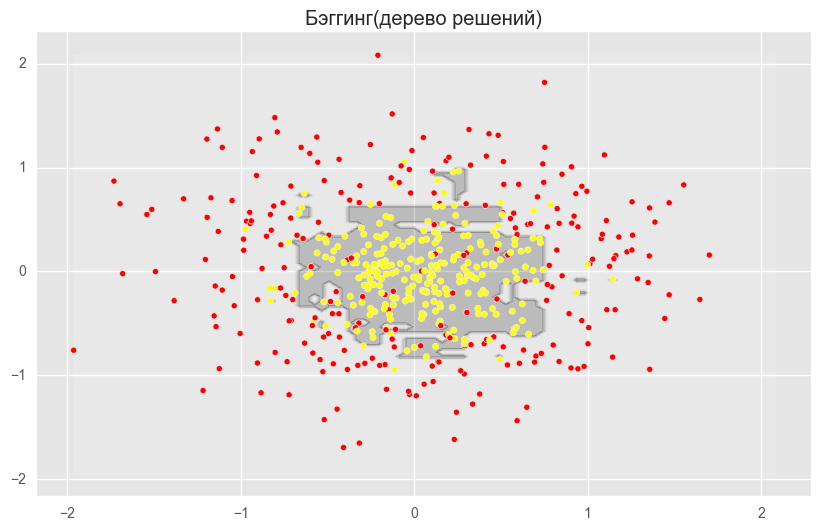
\includegraphics[width=1 \textwidth]{img/bagging_cl}
    \caption{Граница сглаженная и практически нет признаков переобучения}
  \end{figure}
\end{frame}

\begin{frame}{Ошибка out-of-bag}
  \begin{itemize}
    \item Дерево $b_{n}$, обученное с помощью bootstrap, использует в
      среднем $2/3$ наблюдений.
    \item Оставшиеся $1/3$ наблюдений, которые не вошли в
      bootstrap-выборку $\mathbf{X}_{n}$, являются контрольными для
      данного дерева.
    \item Значит, можно для каждого объекта $x_{i}$ найти деревья,
      которые были обучены без него, и вычислить по их ответам
      out-of-bag ошибку:
      \begin{flalign*}
        OOB = \displaystyle\sum_{i =
        1}^{l}L\left(y_{i},\;\frac{1}{\displaystyle\sum_{n =
          1}^{N}[x_{i}\notin\mathbf{X}_{n}]}\displaystyle\sum_{n =
        1}^{N}[x_{i}\notin\mathbf{X}_{n}]b_{n}(x_{i})\right),
      \end{flalign*}
      где $L(y,\; z)$~--- функция потерь.
  \end{itemize}
\end{frame}

\begin{frame}{Random forest}
  Модель \textbf{Random Forest} --- улучшение бэггинга решающих
  деревьев. Деревья становятся менее коррелированными благодаря тому,
  что при построении дерева в каждой вершине признак выбирается из
  случайного подмножества заданного размера $p$.
  \par\smallskip
  Практическая рекомендация: для классификации~--- $p=\sqrt{d}$, где
  $d$ --- общее число признаков; для регрессии~--- $p = d / 3$.
  \par\smallskip
  Ограничения в построении дерева выбираются так, чтобы деревья
  получались глубокими --- такие деревья имеют низкое смещение.
  \par\smallskip
  Количество деревьев может быть определено по графику ошибок от
  числа деревьев. Также стоит учесть вычислительную сложность, хотя
  случайный лес хорошо параллелится.
\end{frame}

\begin{frame}{Random forest в задаче регрессии}
  \begin{figure}[h!]
    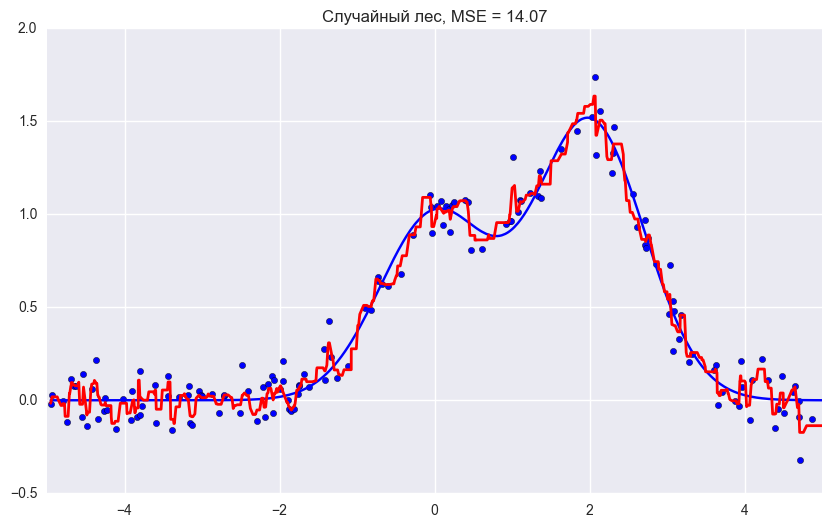
\includegraphics[width=0.8 \textwidth]{img/rf_re}
    \caption{Различие случайного леса и бэггинга на деревьях решений
      заключается в том, что в случайном лесе выбирается случайное
      подмножество признаков, и лучший признак для разделения узла
      определяется из подвыборки признаков, в отличие от бэггинга, где
    все функции рассматриваются для разделения в узле}
  \end{figure}
\end{frame}

\begin{frame}{Random forest в задаче классификации}
  \begin{figure}[h!]
    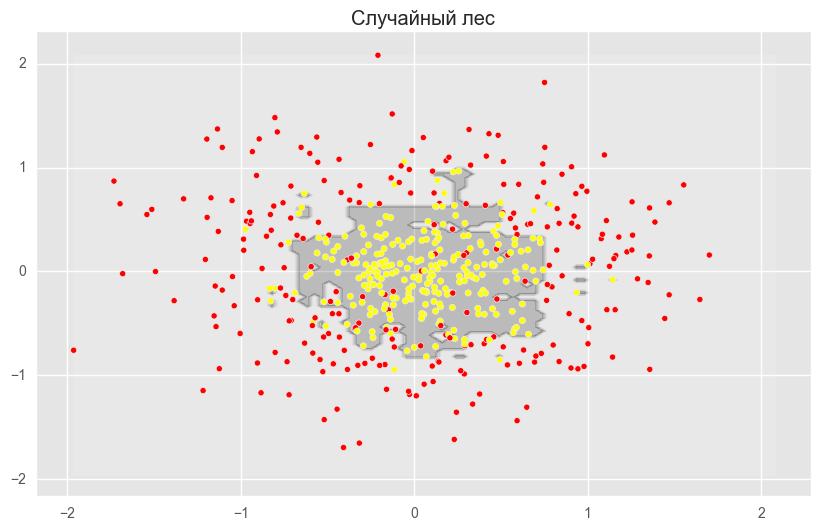
\includegraphics[width=1 \textwidth]{img/rf_cl}
    \caption{Граница сглаженная и практически нет признаков переобучения}
  \end{figure}
\end{frame}

\begin{frame}{Boosting}
  \textbf{Boosting}~--- техника последовательного обучения множества
  слабых базовых моделей для построения более качественной общей
  модели предсказания. В этом случае используется одно обучающее
  множество. Первая модель в последовательности обучается
  предсказывать, а последующие стремятся уменьшить ошибки
  предсказания предыдущих.
  \par\smallskip
  В итоге получаем аддитивную модель как взвешенную
  последовательность множества базовых.
  \par\smallskip
  Рассмотрим в общем виде \textbf{Gradient Boosting} для задачи
  регрессии и \textbf{AdaBoost} для задачи классификации.
\end{frame}

\begin{frame}{Gradient Boosting для задачи регрессии}
  В качестве базовой модели берем дерево решений. Boosting использует
  комбинацию большого количества деревьев. Деревья строятся
  последовательно, при этом  каждое следующее дерево использует
  информацию предыдущих деревьев.
  \par\smallskip
  \textbf{Алгоритм}:
  \begin{enumerate}
    \item Устанавливаем $b(x) = 0$ и $r_{i} = y_{i}$ для всех $i$ на
      обучающем множестве $(\mathbf{X},\; r)$.
    \item Для $n = 1,\; 2,\; \dots,\; N$ повторяем:
      \begin{itemize}
        \item Обучаем дерево $b_{n}$ с $d$ сплитами ($d + 1$
          терминальных узлов) на обучающем множестве $(\mathbf{X},\; r)$.
        \item Обновляем $b$: $b(x) \gets b(x) + \lambda b_{n}(x)$
        \item Обновляем остатки: $r_{i} \gets r_{i} - \lambda b_{n}(x_{i})$
      \end{itemize}
    \item Возвращаем модель:
      \begin{flalign*}
        b(x) = \displaystyle\sum_{n = 1}^{N} \lambda b_{n}(x).
      \end{flalign*}
  \end{enumerate}
\end{frame}

\begin{frame}{Gradient Boosting для задачи регрессии: основная идея}
  Заметим, что мы обучаемся на антиградиент (пусть $\lambda = 1$):
  \begin{flalign*}
    r_i = y_i - b (x_i) = -\frac {d} {dz} \frac {1} {2}(z - y _i) ^2|
    _{z = b (x_i)}
  \end{flalign*}
  \par\smallskip
  \textbf{Идея}: предсказание следующего алгоритма должно быть
  противоположно производной $L(y, z)$ в точке $z=b (x_i)$. Тогда
  вектор сдвигов совпадает с антиградиентом $L$.
  \par\smallskip
  Таким образом, добавляя новый алгоритм, мы делаем шаг градиентного
  спуска. А $\lambda$ является learning rate.
\end{frame}

\begin{frame}{Gradient Boosting для задачи регрессии}
  Три настраиваемых параметра:
  \begin{enumerate}
    \item Количество деревьев $N$. При слишком большом значении $N$
      может привести к переобучению. Можно использовать
      кросс-валидацию для выбора $N$.
    \item Параметр регуляризации $\lambda$~--- небольшое
      положительное число, которое контролирует скорость обучения.
      При очень малом значении $\lambda$ необходимо использовать
      очень большое значение $N$, чтобы получить приемлимый результат.
    \item Количество сплитов $d$ в каждом дереве. Параметр определяет
      сложность ансамбля.
  \end{enumerate}
\end{frame}

\begin{frame}{AdaBoost для задачи классификации}
  \textbf{Общая идея}:
  \begin{itemize}
    \item Последовательно строим модель на базе слабых
      классификаторов при этом уменьшаем ошибку классификатора на
      предыдущем шаге.
    \item Если на обучающем множестве были случаи неправильной
      классификации, то для этих наблюдений увеличивается вес.
    \item Следующий классификатор при обучении использует эти веса,
      чтобы сделать акцент на случаях, где была ошибка.
    \item После этого обученный классификатор может сам давать
      ошибочные классификации, что ведет к изменению весов наблюдений
      для последующего классификатора.
    \item Каждый классификатор в последовательности имеет свой вес.
    \item Таким образом, получаем конечный классификатор как линейную
      комбинацию последовательно обученных классификаторов.
  \end{itemize}
\end{frame}

\begin{frame}{AdaBoost для задачи классификации}
  \textbf{Алгоритм}:
  \begin{enumerate}
    \item Инициализация весов наблюдений $w_{i} = \frac{1}{n}$
      где $i = 1,\; 2,\; \dots,\; n$.
    \item for $m = 1$ to $M$:
      \begin{itemize}
        \item Обучение классификатора $T_{m}(x)$ на обучающих данных
          с весами $w_{i}$.
        \item Вычисление ошибки: $err_{m} = \frac{\sum_{i =
            1}^{n}w_{i} \mathbf{1}\left(y_{i} \neq
          T_{m}(x_{i})\right)}{\sum_{j = 1}^{n}w_{j}}$.
        \item Вычисление веса классификатора $G_{m}(x)$: $\alpha_{m}
          = \log \left[\frac{1 - err_{m}}{err_{m}} \right] + \log(K -
          1)$, где $K$~--- количество классов.
        \item Обновление весов $w_{i} \gets w_{i} \times
          \exp(\alpha_{m}   \times \mathbf{1}(y_{i} \neq T_{m}(x_{i})))$.
        \item Нормализация весов $w_{i}$.
      \end{itemize}
    \item $C(x) =
      \underset{k}{\operatorname{argmax}}\left\{\displaystyle\sum_{m
      = 1}^{M}\alpha_{m} \times \mathbf{1}(T_{m}(x) = k)\right\}$.
  \end{enumerate}
\end{frame}

\begin{frame}{Заключение}
  В \textbf{Random forest}:
  \begin{itemize}
    \item Используются глубокие деревья, так как от базовых
      алгоритмов требуется низкое смещение.
    \item Разброс устраняется за счет усреднения ответов различных деревьев.
  \end{itemize}
  \par\smallskip
  В \textbf{Boosting}:
  \begin{itemize}
    \item Каждый следующий алгоритм понижает ошибку композиции.
    \item Переобучение при большом количестве базовых моделей.
    \item Можно понизить смещение моделей, но разброс или останется
      таким же, или увеличится.
    \item Используются неглубокие решающие деревья.
  \end{itemize}
\end{frame}

\end{document}
